\chapter{Funções}\label{cap:Funcoes}

\epigraph{``Nada que vale a pena é fácil''.}{Eric Cartman,  South Park}

\epigraph{``O ego é o pior inimigo do Eu, mas o Eu é o melhor amigo do ego... O ego é um péssimo senhor, mas é um ótimo servidor''.}{Bhagavad Gita}

\section{Conceitos, Definições e Nomenclaturas}\label{sec:FuncoesConceitoDefinicaoNomenclaturas}

Após o conceito importantíssimo de conjunto o componente mais importante na matemática é provavelmente a noção de função, o autor deste manuscrito não hesita em afirmar que você leitor com certeza já teve contato com a ideia de função, seja em seus curso do primário, secundário ou mesmo mais recentemente em suas disciplinas de nível superior tais como cálculo diferencial e integral ou alguma disciplina de física. Dado este encontra anterior com o assunto o autor fica confortável a pedir que leitor faça uma pequena pausa e tente lembrar de seus cursos anteriores e respondo para si mesmo ao questionamento: \textbf{o que é uma função}?

Bem para muitos físicos, estatísticos e alguns matemáticos (não todos), uma função é vista meramente como sendo um mapeamento (ou transformação) entre os elementos de dois conjuntos \cite{abe1991-TC}. Por outro lado, em obras tais como \cite{sussana2010-MD, lipschutz1971-Topo, lipschutz1978-TC, lipschutz2013-MD, Gerard2021discreta} uma função é vista como uma caso particular de relação entre dois conjuntos, ou seja, em última análise para esse grupo de pessoas uma função é exatamente um conjunto\footnote{Para melhor entender essa visão talvez o leitor deva revistar os Capítulos \ref{cap:Conjuntos} e \ref{cap:Relacoes} e revisar as definições apresentadas nos mesmo.}. Já em \cite{edward2019-MD, fmcbook} é apresentado uma visão mais mecanicista da ideia de função, essa visão captura a ideia de função enquanto uma máquina\footnote{Para cientistas da computação máquina e programas são sinônimos.} (ou caixa preta) que transforma as entradas (\textit{inputs}) em saídas (\textit{outputs}), essa visão é ilustrada pela Figura \ref{fig:FuncaoBlackBox}. 

Há também a ideia de função como sendo uma estrutura \cite{judith2021}, com componentes bem estabelecidos. Essa visão é capaz (como será mostrado a seguir) de captura todas as outras ideias de função.  Neste manuscrito formalização da ideia de função como sendo uma estrutura será apresentada de forma gradual trançando paralelos com a linguagem de programação que possuam um sistema de tipos, isso será adotado para tornar o texto mais didático e interessante ao aluno, além disso, irá aproximar os tópicos teóricos (as funções) dos tópicos práticos (programação) cujo leitor desse manuscrito naturalmente tem contato e provável interesse. Entretanto, esse forma de apresentação não será menos rigorosa que outras fontes bibliográficas, na verdade será o oposto, o texto aqui apresentado tende a ser mais preciso e detalhado que a apresentação rasa feita em \cite{judith2021}.

\begin{figure}[h]
	\centering
	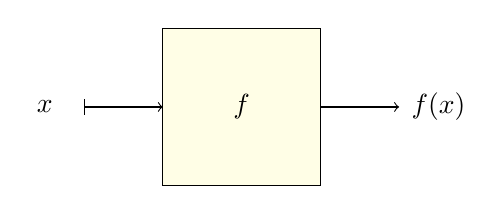
\begin{tikzpicture}
		\draw [rounded corners=0mm, fill=yellow!10]  (-1,1)--(-1,-1)--(1,-1)--(1,1)--cycle;
		\draw[->]  (1.0,0) -- (2.0,0.0);
	    \draw[|->]  (-2.0,0) -- (-1.0,0.0);
		\node (f) at (0,0) {$f$};
		\node (fx) at (2.5,0) {$f(x)$};
		\node (x) at (-2.5,0) {$x$};
	\end{tikzpicture}
	\caption{Visão de uma função de uma variável enquanto uma máquina (ou caixa preta).}
	\label{fig:FuncaoBlackBox}
\end{figure}

Este manuscrito irá iniciar o estudo sobre funções  apresentado ao leitor a ideia básica de assinatura de função, isto é, a seguir será apresentado a estrutura sintática das funções.

\begin{definition}[Assinatura de Função]\label{def:AssinaturaFuncao}
	Sejam $A$ e $B$ conjuntos a assinatura da função de $A$ em $B$ nomeada como $f$ corresponde a uma palavra da forma $f: A \rightarrow B$.
\end{definition}

Note que a Definição \ref{def:AssinaturaFuncao} permite facilmente deduzir que em qualquer função existem três componentes básicos, sendo eles: um nome (ou rótulo), um conjunto de partida e um conjunto de chegada. 

% Susam, lipstick (topo),  ver como relação